\documentclass[12pt,a4paper]{article}
\usepackage[spanish]{babel}
\usepackage[utf8]{inputenc}
\usepackage{hyperref}
\usepackage{float}
\usepackage{geometry}
\usepackage{xcolor}
\usepackage{array}
\usepackage{longtable}
\usepackage{chngcntr}
\counterwithin{figure}{section}
\counterwithin{table}{section}
\usepackage{graphicx}
\usepackage{fancyhdr}
\usepackage{adjustbox}


% Definimos el color de los meses y líneas
\definecolor{mescolor}{HTML}{024d50}
\definecolor{linecolor}{HTML}{024d50}

% Cambiar color de secciones (meses)
\usepackage{titlesec}
\titleformat{\section}
  {\color{mescolor}\normalfont\Large\bfseries}
  {}{0pt}{}
\titlespacing*{\section}{0pt}{*2}{*1}

% Línea negra debajo de cada mes
\newcommand{\separador}{\vspace{0.5cm}\noindent\rule{\linewidth}{0.5pt}\vspace{0.5cm}}

% Cambiar color en el índice y tamaño más grande
\usepackage{tocloft}
\renewcommand{\cftsecfont}{\color{mescolor}\bfseries\Large}
\renewcommand{\cftsecpagefont}{\color{mescolor}\bfseries\Large}

% Configuración encabezado y pie de página con líneas de color y largo ajustable
\pagestyle{fancy}
\fancyhf{}
\fancyhead[L]{\textbf{Proyecto BlindAssist}} % encabezado solo a la izquierda
\fancyhead[R]{\includegraphics[width=0.08\linewidth]{Carpeta de campo/logo indice.png}} % no mostrar nada a la derecha
\fancyfoot[C]{\thepage} % pie centrado

% Línea de encabezado de color y largo personalizado
\renewcommand{\headrulewidth}{0.4pt} % grosor (puedes cambiarlo)
\renewcommand{\footrulewidth}{0.4pt} % grosor (puedes cambiarlo)

\renewcommand{\headrule}{%
  \color{linecolor}\hrule width 1\linewidth height 0.4pt \vskip0pt} % 0.8\linewidth = largo de la línea
\renewcommand{\footrule}{%
  \color{linecolor}\hrule width \linewidth height 0.4pt \vskip0pt} % 0.6\linewidth = largo del pie
\begin{document}

% Carátula (imagen jpg ocupa toda la primera página, sin número)
\clearpage
\newgeometry{top=0cm,bottom=0cm,left=0cm,right=0cm}
\thispagestyle{empty}
\begin{figure}[!t]
    \centering
    \includegraphics[width=\paperwidth,height=\paperheight]{Carpeta de campo/caratula campo.jpg}
\end{figure}
\restoregeometry
\clearpage
% Índice con numeración desde aquí
\setcounter{page}{1}
\tableofcontents
\begin{figure}[h]
    \centering % centra la imagen
    \includegraphics[width=0.7\linewidth]{Carpeta de campo/logo indice.png} % ancho relativo al texto
\end{figure}
\newpage

%---------------------------------------------------
\section*{Abril 2025}
\addcontentsline{toc}{section}{Abril 2025}

\subsection*{14-19 Abril}
Definimos el branding del proyecto, aprendimos los conceptos básicos de git y github, realizamos cursos de Python, además de cursos de HTML, realizamos un wireframe básico de la página web, investigación de los sensores LIDAR a utilizar.

\textbf{Tiago Quattrocchi:} Curso de Python (6h) e investigación sensor LIDAR (2h).  

\textbf{Pino:} Curso de HTML y CSS (1h aprox). Wireframe en Figma (10 min). Branding general (50 min). Curso Python (6h).  

\textbf{Ramiro Castillo:} Curso básico de HTML y CSS (4h). Práctica de ejercicios (1h 30m). Participación en branding (30 min).

\begin{figure}[H]
    \centering
    \includegraphics[width=0.5\linewidth]{Carpeta de campo/logo.jpg}
    \label{fig:placeholder}
\end{figure}

\begin{figure}[H]
\centering
    \includegraphics[width=0.5\linewidth]{Carpeta de campo/Tfmini invest.png}
    \label{fig:placeholder}
\end{figure}

\subsection*{22-27 Abril}
Producimos un listado de las posibles empresas sponsor, envío de mails a sponsors, wireframe web casi completo, organización del repositorio para trabajar de manera ordenada y profesional, reunión con director de Biblioteca Braille de Bahía Blanca (2h), programación de la web, familiarizacion con la app Trello, finalización branding.

\textbf{Ramiro Castillo:} Reunión (2h), envío de mails (10 min), investigación sobre JS (1h), programación en HTML/CSS/JS (4h) de la página web.  

\textbf{Pino:} Reunión (2h), mails (10 min), finalización de branding (3h), accesibilidad Instagram (30 min), backlog en Notion (30 min), creación de reel (1h).  

\textbf{Tiago:} Reunión con Biblioteca Braille (2h), organización Trello (1h).

\begin{figure}[H]
    \centering
    \begin{minipage}{0.45\textwidth}
        \centering
        \includegraphics[width=\linewidth]{Carpeta de campo/Imagen2.jpg}
    \end{minipage}
    \hfill % espacio entre imágenes
    \begin{minipage}{0.45\textwidth}
        \centering
        \includegraphics[width=\linewidth]{Carpeta de campo/Imagen3.jpg}
    \end{minipage}
\end{figure}
\includegraphics[width=\linewidth]{Carpeta de campo/Imagen4.jpg}

\begin{figure}
    \includegraphics[width=0.5\linewidth]{Carpeta de campo/Reunion.png}
\end{figure}

\subsection*{29 Abril - 3 Mayo}

\begin{itemize}
    
\item Organización del excel de componentes para realizar las compras a cooperadora.

\begin{figure}[H]
    \includegraphics[width=\linewidth]{Carpeta de campo/Excel.png}
\end{figure}

\item Escribimos carta para Globant para pedir sponsor intelectual (acerca del funcionamiento de una IA y su desarrollo ) o economico. 

\item Enviamos mails a empresas locales manteniendo un formato formal en el que solicitamos ayuda economica.
\begin{figure}[H]
    \includegraphics[width=1\linewidth]{Carpeta de campo/Mail.png}
\end{figure}

\item Cálculo del costo de los materiales. 

\item Elección de baterías de acuerdo a nuestro presupuesto y necesidad.

\item Pruebas iniciales de los sensores TFmini en Python.

\end{itemize}


%---------------------------------------------------
\separador
\section*{Mayo 2025}
\addcontentsline{toc}{section}{Mayo 2025}



\includegraphics[width=\linewidth]{Carpeta de campo/Imagen6.png}

\subsection*{5-9 Mayo}

\begin{itemize}
    
\item Selección de cámara con una buena relación calidad-precio.
\item Cálculo de consumo y selección de baterías de litio.
\item Seguimos enviando mails a posibles sponsors.

\end{itemize}
\includegraphics[width=0.5\linewidth]{Carpeta de campo/Imagen7.png}
\includegraphics[width=0.5\linewidth]{Carpeta de campo/Imagen8.png}

\subsection*{12-16 Mayo}
\begin{itemize}

\item Realizamos prácticas profesionalizantes  de Newton.
\item Realizamos prácticas profesionalizantes en UTN.
\item Investigación detección de obstáculos con el uso de IA.
\item Realización de un curso básico de AutoCAD.
\begin{figure}[H]
    \centering
    \includegraphics[width=\linewidth]{Carpeta de campo/Curso AutoCad.png}
\end{figure}
\item Investigación de códigos de prueba para medir distancias con TFMini LIDAR.

\includegraphics[scale=1]{Carpeta de campo/Imagen9.png}
\end{itemize}

\subsection*{19-23 Mayo}

\begin{itemize}
\item Realizamos prácticas profesionalizantes en Newton y UTN.
\item Empezamos el entrenamiento de la IA de detección de objetos desde cero.
\item Actualización/hosteo de la página web.
\begin{figure}[H]
\includegraphics[width=\linewidth]{Carpeta de campo/Imagen10.png}
\end{figure}
\item Preparación para la inspección.



\item Subir código a Raspberry Pi 4 mediante el programa Termius.
\begin{figure}[H]
    \centering
    \includegraphics[width=0.75\linewidth]{Carpeta de campo/Subir a Termius.png}
\end{figure}
\item Realizamos mediciones y cálculos de dimensiones generales del proyecto.

\end{itemize}

\subsection*{26-30 Mayo}

\begin{itemize}

\item Salida educativa a UADE (martes sin actividad).
\end{itemize}

\separador

%---------------------------------------------------
\section*{Junio 2025}
\addcontentsline{toc}{section}{Junio 2025}

\subsection*{2-6 Junio}
\begin{itemize}
\item Realizamos prácticas UTN.
\item Investigación de múltiples UARTs por software en la Raspberry Pi 4.

\begin{figure}[H]
    \centering
    \includegraphics[width=0.75\linewidth]{Carpeta de campo/Softuart.png}
\end{figure}

\item Realización de curso basico de Kicad.
\item Primeras pruebas de código subido en la Raspberry Pi4.

\includegraphics[width=0.7\linewidth]{Carpeta de campo/Imagen11.png}
\end{itemize}

\subsection*{9-13 Junio}
\begin{itemize}

\item Realizamos prácticas en la UTN 
\item Iniciamos contacto con posibles patrocinadores para el proyecto.

\begin{figure}[H]
    \centering
    \includegraphics[width=0.5\linewidth]{Carpeta de campo/Colaboración.png}

\end{figure}

\item Investigación de alimentación adecuada y segura tanto para la Raspberry Pi 4 como la placa de componentes en general.

\begin{figure}[H]
    \centering
    \includegraphics[width=0.5\linewidth]{Carpeta de campo/Cable usb c.png}
\end{figure}

\item Primera prueba de implementación de UART por software.

\end{itemize}

\includegraphics[width=0.6\linewidth]{Carpeta de campo/Imagen12.png}

\includegraphics[width=0.7\linewidth]{Carpeta de campo/Imagen13.png}

\subsection*{16-20 Junio}

\begin{itemize}
\item Investigación para optimizar el código mediante programación orientada a objetos.
\begin{figure}[H]
    \centering
    \includegraphics[width=0.7\linewidth]{Carpeta de campo/Imagen14.png}
\end{figure}



\item Solución de problemas de alimentación de la Raspberry Pi 4.
\begin{figure}[H]
\centering
\includegraphics[width=0.5\linewidth]{Carpeta de campo/Imagen15.png}
\end{figure}
\end{itemize}

\subsection*{23-27 Junio}

\begin{itemize}

\item Cerramos acuerdo con el la empresa para oficializar el sponsor (TodoMicro).

\item Charla con sponsor para entrega de componentes.

\includegraphics[width=0.7\linewidth]{Carpeta de campo/Imagen16.png}
\includegraphics[width=0.2\linewidth]{Carpeta de campo/Imagen17.png}

\item Investigación y prueba de adaptador TTL-USB (reemplazo al UART por software).

\includegraphics[width=0.7\linewidth]{Carpeta de campo/Imagen18.png}

\end{itemize}

%---------------------------------------------------
\separador

\section*{Julio 2025}
\addcontentsline{toc}{section}{Julio 2025}

\subsection*{30 Junio - 4 Julio}
\begin{itemize}
\item Realización del primer modelo 3D básico en base a sketch realizado (primeros prototipos).
\begin{figure}[H]
    \centering
    \includegraphics[width=0.75\linewidth]{Carpeta de campo/Imagen20.jpg}
    \label{fig:placeholder}
\end{figure}
\includegraphics[width=\linewidth]{Carpeta de campo/Imagen21.jpg}
\item Planteamiento de publicaciones de sponsor (reels y storys). 
\item Escribimos un nuevo codigo mejorado para la medición de distancia mediante los LIDAR.

\includegraphics[width=0.7\linewidth]{Carpeta de campo/Imagen19.png}

\item Primeras pruebas con la Deteccion de objetos por IA.

\begin{figure}
    \centering
    \includegraphics[width=0.5\linewidth]{Carpeta de campo/Deteccioncam.png}
\end{figure}


\end{itemize}

\subsection*{7-11 Julio}
\begin{itemize}

\item Realizamos prácticas en Fuerza Aérea.
\item Coordinación de entrega de productos con el sponsor.
\item Organización de reel para oficializar el sponsor.
\begin{figure}[H]
    \centering
    \includegraphics[angle=90, width=0.75\linewidth]{Carpeta de campo/Reeltodomicro.png}
\end{figure}

\end{itemize}

\subsection*{14-18 Julio}

\begin{itemize}
\item Prácticas en Fuerza Aérea. 
\item Retiro de productos en sponsor.

\item Grabar reel de presentación de sponsor.
\begin{figure}[H]
    \centering
    \includegraphics[width=0.75\linewidth]{Carpeta de campo/Reel sponsor.png}
\end{figure}
\item Grabar reel de muestra de los productos.
\begin{figure}[H]
    \centering
    \includegraphics[width=0.75\linewidth]{Carpeta de campo/reelcomp.png}
\end{figure}
\item Editar ambos reel de sponsor.
\end{itemize}

\separador

%---------------------------------------------------
\section*{Agosto 2025}
\addcontentsline{toc}{section}{Agosto 2025}

\subsection*{4-8 Agosto}

\begin{itemize}
\item Realizamos prácticas en Newton.
\item Idear fijaciones de los componentes a la carcasa.
\item Investigación de cómo implementar programación orientado a objetos en python.
\begin{figure}[H]
\includegraphics[width=\linewidth]{Carpeta de campo/Imagen22.png}
\end{figure}

\end{itemize}

\subsection*{11-15 Agosto}
\begin{itemize}
\item Realizamos prácticas en Newton.
\item Preparación entorno virtual de Python para aislar dependencias.
\item Idear fijaciones y straps a las tapas de la carcasa.
\end{itemize}

\subsection*{18-22 Agosto}
\begin{itemize}
\item Realizamos prácticas en Newton.

\item Diseño del primer esquemático en proteus 8.

\begin{figure}[H]
    \centering
    \includegraphics[width=0.75\linewidth]{Carpeta de campo/Captura de pantalla (1).png}
\end{figure}

\item Diseño de la primera PCB teniendo en cuenta los componentes que se van a utilizar y como va a estar ubicada dentro de la carcasa.

\begin{figure}[H]
    \centering
    \includegraphics[width=0.75\linewidth]{Carpeta de campo/Captura de pantalla (2).png}
\end{figure}

\item Arreglo código de TFmini, cambiando la estructura de lectura UART.

\includegraphics[width=0.7\linewidth]{Carpeta de campo/imagen 31.png}

\item Impresión de la primera carcasa.
\end{itemize}

\begin{figure}[H]
    \centering
    \includegraphics[width=0.4\linewidth]{Carpeta de campo/primera carcasa.jpg}
\end{figure}

\subsection*{25-29 Agosto}
\begin{itemize}

\item Arreglo de los conectores rotos de TFmini.

\includegraphics[width=0.5\linewidth]{Carpeta de campo/imagen29.png}

\item Pruebas individuales de cada TFmini con el software oficial de Benewake.

\includegraphics[width=0.5\linewidth]{Carpeta de campo/imagen30.png}

\item investigación del modulo RP2040 Zero.

\begin{figure}[H]
    \centering
    \includegraphics[width=0.5\linewidth]{Carpeta de campo/RP2040.png}
\end{figure}

\item Rediseño conceptual del prototipo (preparación de la  versión 2).

\item Diseñamos un nuevo modelo 3D (prototipo) teniendo en cuenta los cambios en las proporciones y la angulación de los sensores.

\begin{figure}[H]
    \centering
    \includegraphics[width=0.75\linewidth]{Carpeta de campo/segundo proto.png}
\end{figure}

\item Primeras pruebas de adaptación del código de detección por IA a programación orientada a objetos.


\end{itemize}


\separador

%---------------------------------------------------
\section*{Septiembre 2025}
\addcontentsline{toc}{section}{Septiembre 2025}

\subsection*{1-5 Septiembre}
\begin{itemize}
\item Solución de problemas de conexión SSH en Raspberry Pi 4 (utilizamos una red local para que se haga transportable la comunicación SSH, además de más segura al usar una red con únicamente 2 direcciones IP).


\item Reorganización del GitHub a un modelo mas formal y mejor estructurado.

\begin{figure}[H]
    \centering
    \includegraphics[width=0.5\linewidth]{Carpeta de campo/Imagen23.png}
\end{figure}


\end{itemize}

\subsection*{8-12 Septiembre}
\begin{itemize}
\item Prueba de código POO (unicamente la detección de objetos).

\begin{figure}[H]
    \centering
    \includegraphics[width=0.5\linewidth]{Carpeta de campo/Camara.png}
\end{figure}
\item Solución de problemas de dependencias en Raspbian.
\item Realizamos un test de audio en la Raspberry Pi 4 utilizando el jack integrado.

\begin{figure}[H]
    \centering
    \includegraphics[width=0.4\linewidth]{Carpeta de campo/Audio.png}
\end{figure}
\item Realizamos pruebas con 3 TFmini secuenciales y realizando detección de distancia al mismo tiempo.

\begin{figure}[H]
    \centering
    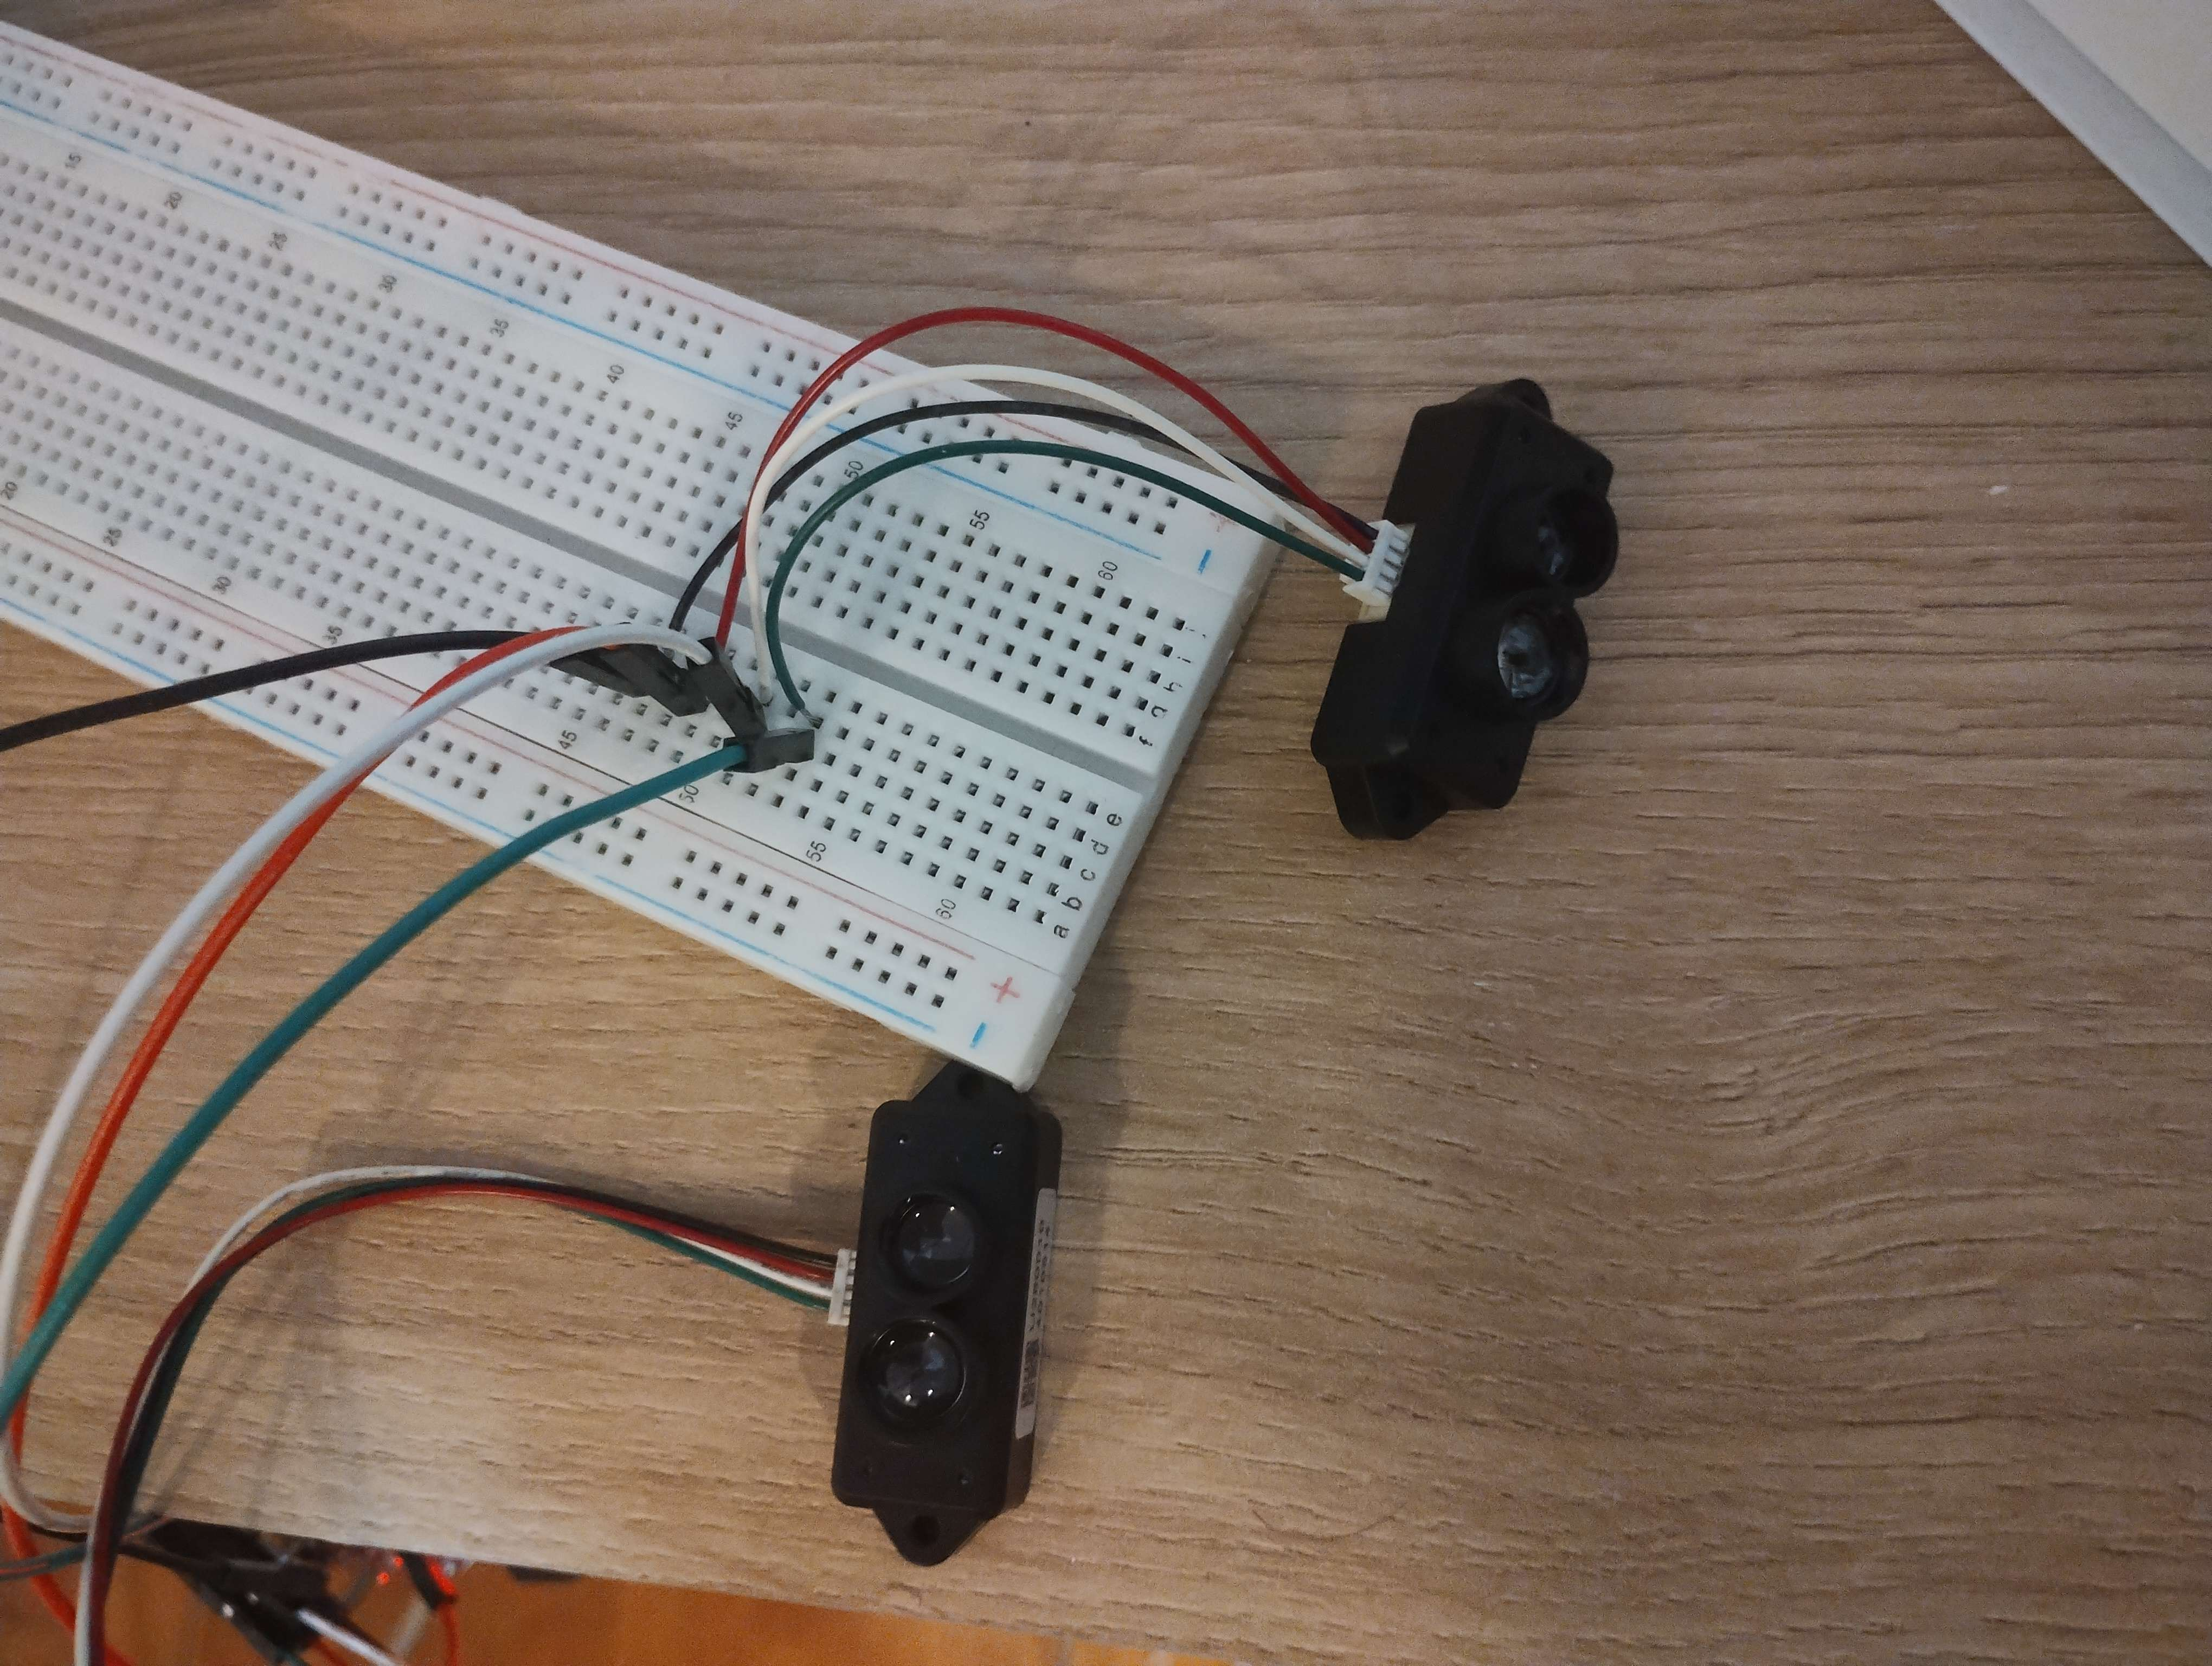
\includegraphics[width=0.5\linewidth]{Carpeta de campo/Tres TF.png}
\end{figure}
\item Comprobamos el funcianomiento de los pines de PWM de la Raspberrry Pi 4 mediante LEDs.
\item Combinación de los códigos de detección por Ia y detección de distancia por TFmini en un codigo de POO (Programación orientada a objetos).


\includegraphics[width=0.7\linewidth]{Carpeta de campo/Imagen24.png}

\includegraphics[width=0.7\linewidth]{Carpeta de campo/imagen28.png}


\end{itemize}
\subsection*{15-19 Septiembre}

\begin{itemize}
\item Actualización de las carpetas tanto técnicas como de campo al formato de ONIET.

    \includegraphics[width=0.5\linewidth]{Carpeta de campo/Carpcampo.png}
    \includegraphics[width=0.5\linewidth]{Carpeta de campo/Carptec.png}



\item Finalización de código de POO con detección por cámara.

\item Rediseño de PCB, cambiando la organización de la alimentación, implementando un mejor manejo de masa y la distribución de las pistas.

\begin{figure}[H]
    \centering
    \includegraphics[width=0.75\linewidth]{Carpeta de campo/PCB2.png}
\end{figure}

\item Probamos el control de PWM en un entorno virtual dentro de la Raspberry, probamos físicamente el código con un motor y un LED.
\begin{figure}[H]
    \centering
    \includegraphics[width=0.5\linewidth]{Carpeta de campo/PWM prueba.png}
\end{figure}

\item Impresión de la segunda versión de la  carcasa.
\begin{figure}[H]
    \centering
    \includegraphics[width=0.4\linewidth]{Carpeta de campo/Impresion 2.png}
\end{figure}

\begin{figure}[H]
    \centering
    \includegraphics[width=0.4\linewidth]{Carpeta de campo/Segunda carcasa.jpg}
\end{figure}

\item Rediseño interior de la carcasa adaptándose al tamaño real de los TFmini (Hubo un error en la segunda versión en la cual no había espacio para los sensores de distancia).

\begin{figure}[H]
    \centering
    \includegraphics[width=0.5\linewidth]{Carpeta de campo/Tapa 2.png}
\end{figure}

\item Realizamos la organización de una mejor distribución de los espacios dentro de la carcasa.

\begin{figure}[H]
    \centering
    \includegraphics[width=0.4\linewidth]{Carpeta de campo/Distribución.png}
\end{figure}
\item Adaptar carpeta técnica al formato de ONIET.
\item Adaptar carpeta de campo al formato de ONIET.

\includegraphics[width=0.7\linewidth]{Carpeta de campo/Imagen27.png}
\end{itemize}

\subsection*{22-26 Septiembre}

\begin{itemize}
\item Diseñar base del banner para la muestra en ONIET y la feria de fin de año.

\item Terminamos el diseño final del banner teniendo en cuenta los parámetros requeridos.

\includegraphics[width=0.5\linewidth]{Carpeta de campo/banner.png}
    
\item Probar funcionamiento de motores con esquema circuital planteado.

\item Tercer rediseño de la carcasa superior. Corregido de ángulos interiores.


    
\item Arreglar problema de medición de los TFmini forzando el bit de lectura de distancia.

\includegraphics[width=0.5\linewidth]{Carpeta de campo/arreglomed.png}

\item Adaptar código de medición al feedback de las pruebas realizadas.

\includegraphics[width=0.5\linewidth]{Carpeta de campo/lgicaact.png}
    
\item Impresión de tapa inferior y superior de la tercera versión de la carcasa.
\end{itemize}

\separador

\section*{Octubre 2025}
\addcontentsline{toc}{section}{Octubre 2025}

\subsection*{29 Septiembre - 3 Octubre}

\begin{itemize}
\item Cortar cable de alimentación USB-C.
\item Agregar interruptor de encendido al conexionado.

\includegraphics[width=0.5\linewidth]{Carpeta de campo/interruptor.png}

\item Actualizamos el código de la lógica haptica, cambiando las distancias y la forma en que se maneja el control para conseguir una mejor orientacion al usarlo.
\item Impresión de la primera placa de prototipo.
\end{itemize}

\subsection*{6-10 Octubre}
\begin{itemize}
\item Soldadura de componentes a la placa.

    \includegraphics[width=0.5\linewidth]{Carpeta de campo/soldadura.png}

\item Prueba con la placa completa de ambos códigos.
\item Recibimos el banner físico.
\item Realización del informe descriptivo para ONIET.
\begin{figure}[H]
    \centering
    \includegraphics[width=0.5\linewidth]{Carpeta de campo/informe.png}
\end{figure}

\end{itemize}

\subsection*{13-17 Octubre}
\begin{itemize}
\item Limpieza y reorganización de componentes en la placa.

    \includegraphics[width=0.5\linewidth]{Carpeta de campo/placa limpia.png}

\item Agregamos protecciones de alimentación en la placa.

\item Realizamos la organización de la ubicación de los componentes dentro de la carcasa.

\begin{figure}[H]
    \centering
    \includegraphics[width=0.75\linewidth]{Carpeta de campo/tapa org.png}
\end{figure}

\begin{figure}[H]
    \centering
    \includegraphics[width=0.75\linewidth]{Carpeta de campo/base org.png}
\end{figure}
\item Fijación de los componentes a la tapa superior e inferior.
\item Realizamos pruebas con el primer prototipo ya armado.

\begin{figure}[H]
    \centering
    \includegraphics[width=0.5\linewidth]{Carpeta de campo/protooniet.jpg}
\end{figure}

\item Impresión de las carpetas para ONIET.

\item Ensamblaje del stand para ONIET

\begin{figure}[H]
    \centering
    \includegraphics[width=0.75\linewidth]{Carpeta de campo/stand.png}
\end{figure}

\item Exposición de proyecto en ONIET

\begin{figure}[H]
    \centering
    \includegraphics[width=0.75\linewidth]{Carpeta de campo/expo.png}
\end{figure}



\end{itemize}

\subsection*{20-24 Octubre}

\begin{itemize}
    \item Diseño de panfletos del proyecto
    \begin{figure}[H]
        \centering
        \includegraphics[width=0.5\linewidth]{Carpeta de campo/panfleto.png}
    \end{figure}
    \item Realizar base del Manual de Usuario

\begin{figure}[H]
    \centering
    \includegraphics[width=0.5\linewidth]{Carpeta de campo/manual.png}
\end{figure}

    \item Escribir guión de video de presentación del proyecto
    \begin{figure}[H]
        \centering
        \includegraphics[width=0.5\linewidth]{Carpeta de campo/image.png}
    \end{figure}
    \item Diseño de agarres del dispositivo

\begin{figure}
    \centering
    \includegraphics[width=0.5\linewidth]{Carpeta de campo/agarres.jpg}
\end{figure}
    
    \item Charla con el sponsor para invitar a la feria
\end{itemize}

\subsection*{27-31 Octubre}

\begin{itemize}
\item Grabar video de presentación del proyecto

\begin{figure}[H]
    \centering
    \includegraphics[angle=270, width=0.5\linewidth]{Carpeta de campo/Setvideo.JPG}
\end{figure}

\item Realizar correcciones de video original
\item Organización del github del proyecto
\item Investigación de inicialización de programa con Raspberry pi 4
\item Edición de video de presentación

\begin{figure}[H]
    \centering
    \includegraphics[width=0.5\linewidth]{edicion.png}
\end{figure}

\item Diseños de instrucciones para el manual de usuario

\begin{figure}[H]
    \centering
    \includegraphics[width=0.5\linewidth]{Carpeta de campo/IA deteccion 3 personas.png}
\end{figure}

\item Finalización del manual de usuario
\end{itemize}

\separador

\section*{Noviembre 2025}
\addcontentsline{toc}{section}{Noviembre 2025}

\subsection*{3-7 Noviembre}
\begin{itemize}
\item Reorganización repositorio Github.
\item Correcciones finales del Video Presentación.
\item Actualización Código Web.
\begin{figure}[H]
    \centering
    \includegraphics[width=0.5\linewidth]{Carpeta de campo/pruebas.jpg}
\end{figure}

\end{itemize}
\subsection*{9-15 Noviembre}
\begin{itemize}
    \item Actualización Redes sociales Profesionales: Linkedin, Youtube.

\begin{figure}[H]
    \centering
    \includegraphics[width=0.6\linewidth]{Carpeta de campo/linkedin.png}
\end{figure}

\begin{figure}[H]
    \centering
    \includegraphics[width=0.6\linewidth]{Carpeta de campo/youtube.png}
\end{figure}
    
    \item Implementación de Botones a la placa.
    \item Implementación de Botones por código.
    \begin{figure}
        \centering
        \includegraphics[width=0.5\linewidth]{Carpeta de campo/botones.png}
    \end{figure}
    \item Actualización Curriculum Vitae.
    \item Preparación del stand para la feria
    \item Exposicion de proyecto en la feria
    \begin{figure}[H]
        \centering
        \includegraphics[width=0.5\linewidth]{Carpeta de campo/expo.png}
    \end{figure}

\end{itemize}

\subsection*{17-21 Noviembre}

\begin{itemize}
    \item Diseñar PowerPoint de presentación
    \begin{figure}[H]
        \centering
        \includegraphics[width=0.5\linewidth]{Carpeta de campo/powerfinal.png}
    \end{figure}
    \item Presentación final del proyecto
    \item Actualización final de carpetas y github
    \begin{figure}[H]
        \centering
        \includegraphics[width=0.5\linewidth]{Carpeta de campo/image.png}
    \end{figure}
\end{itemize}
%---------------------------------------------------
\section*{Facturas}
\addcontentsline{toc}{section}{Facturas}

\begin{figure}[H]
    \centering
    \includegraphics[width=0.9\linewidth]{Carpeta de campo/fact1.jpg}
\end{figure}

\begin{figure}
    \centering
    \includegraphics[width=1\linewidth]{Carpeta de campo/fact2jpg.jpg}
\end{figure}

\begin{figure}
    \centering
    \includegraphics[width=1\linewidth]{Carpeta de campo/fact3.jpg}
\end{figure}

\begin{figure}[H]
    \centering
    \includegraphics[width=1\linewidth]{Carpeta de campo/fact4.jpg}
\end{figure}

\end{document}
